\documentclass[border=3pt,tikz]{standalone}
\usepackage{amsmath}
\usetikzlibrary{calc}
\usetikzlibrary{arrows.meta} % for arrow size
\begin{document}
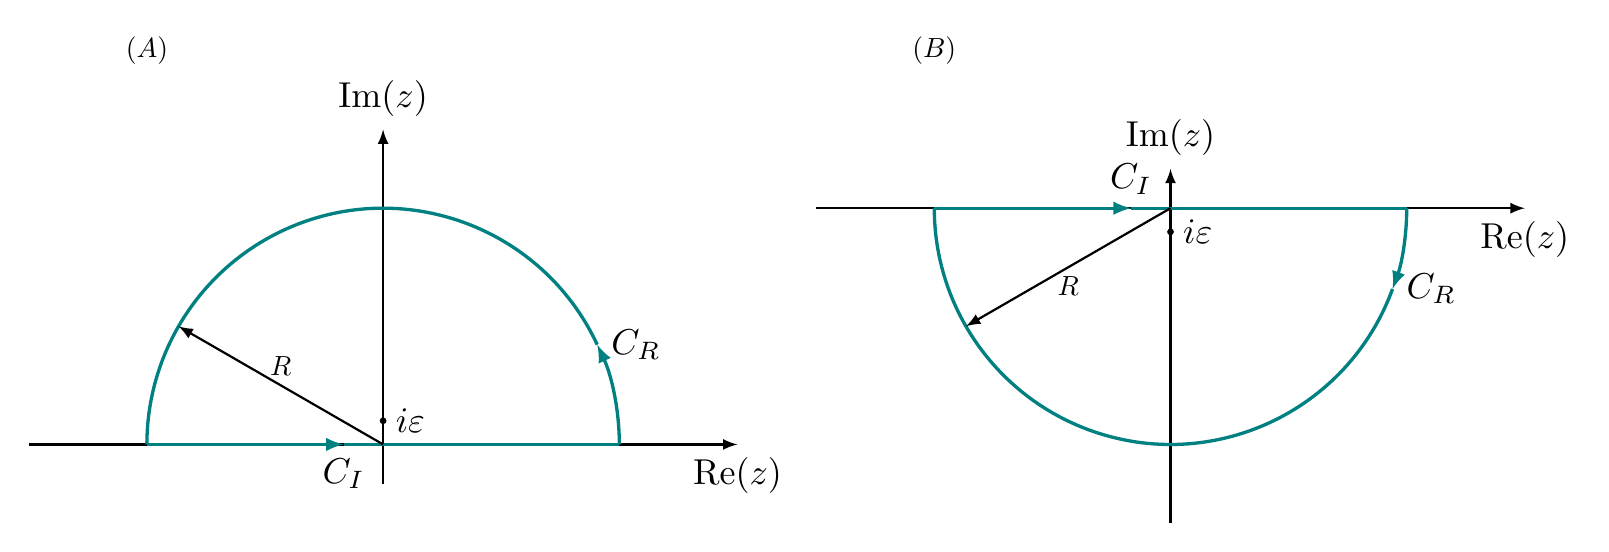
\begin{tikzpicture}[scale=1]
    \usetikzlibrary {arrows.meta}
    \usetikzlibrary {calc}
    
    \node [] at (-3, 5) {$(A)$};
    \draw [thick,-latex] (-4.5, 0) -- (4.5, 0) node[below, scale=1.3] {Re$(z)$};
    \draw [thick, -latex] (0, -0.5) -- (0, 4) node[above, scale=1.3] {Im$(z)$};
    
    \draw[teal, very thick, -latex,] (3, 0) arc (0:25:3) node[black,right, scale=1.3] {$C_R$};
    \draw[teal, very thick,] ({3*cos(25)}, {3*sin(25)}) arc (25:180:3);
    \draw[teal, very thick, -latex] (-3, 0) -- (-0.5, 0) node[black, below, scale=1.3] {$C_I$};
    \draw[teal, very thick] (-0.5, 0) -- (3, 0) ;
    \filldraw[black] (0, 0.3) circle (1pt) node [right, scale = 1.3] {$i\varepsilon$};
    \draw[thick, -latex] (0, 0) -- ({3*cos(150)}, {3*sin(150)});
    \node[above]  at ({1.5*cos(150)}, {1.5*sin(150)}) {$R$};
    
    \begin{scope}[shift={(10,3)}]
    \node [] at (-3, 2) {$(B)$};
    \draw [thick,-latex] (-4.5, 0) -- (4.5, 0) node[below, scale=1.3] {Re$(z)$};
    \draw [thick, -latex] (0, -4) -- (0, 0.5) node[above, scale=1.3] {Im$(z)$};
    
    \draw[teal, very thick, -latex,] (3, 0) arc (0:-20:3) node[black,right, scale=1.3] {$C_R$};
    \draw[teal, very thick,] ({3*cos(-20)}, {3*sin(-20)}) arc (-20:-180:3);
    \draw[teal, very thick, -latex] (-3, 0) -- (-0.5, 0) node[black, above, scale=1.3] {$C_I$};
    \draw[teal, very thick] (-0.5, 0) -- (3, 0) ;
    \filldraw[black] (0, -0.3) circle (1pt) node [right, scale = 1.3] {$i\varepsilon$};
    \draw[thick, -latex] (0, 0) -- ({3*cos(210)}, {3*sin(210)});
    \node[below]  at ({1.5*cos(210)}, {1.5*sin(210)}) {$R$};
    \end{scope}
    \end{tikzpicture}
\end{document}